\subsection{UC-22}
\label{subsec:UC-22}

\begin{figure}[H]
    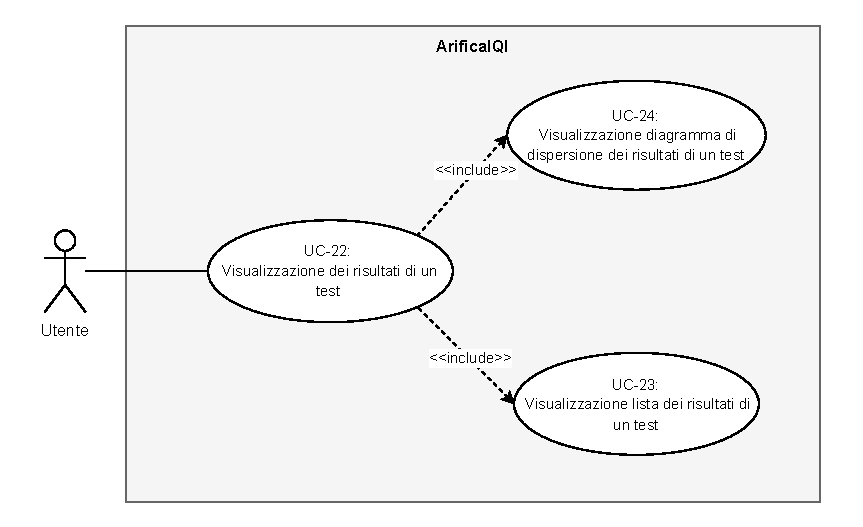
\includegraphics{Sezioni/UseCase/Immagini/UC-22.pdf}
    \caption{Diagramma UC-22.}
\end{figure}

\begin{usecase}{UC-22}{Visualizzazione dei risultati di un test}

    \req{\hyperref[item:RU-8]{RU-8}} 

    \pre{
        \item Il sistema è attivo e funzionante
        \item Sono disponibili i risultati di un test
    }

    \post{
        \item L'utente conosce l'esito del test
    }
    
    \actor{Utente}

    \subactors{}

    \trigger{L'utente deve testare il LLM usando il dataset caricato}
    
    \inc{\hyperref[subsec:UC-23]{UC-23}, \hyperref[subsec:UC-24]{UC-24}}

    \base{}

    \scenario{
        \item \texttt{<<include:UC-23>>}
        \item \texttt{<<include:UC-24>>}
    }

\end{usecase}